% This file describes the general structure of some of our sm_sir models.
% Note that it is possible to construct models in many different ways using the sm_sir code.
% Therefore, this description should be used with caution, because it only describes one possible model configuration.

\section{Model description}

\subsection{General approach}
We use a compartmental model of COVID-19 transmission governed by ordinary differential equations (ODEs). Our model captures
important factors of COVID-19 transmission and disease such as age-specific characteristics, heterogeneous mixing,
vaccination and the emergence of different variants of concern. The ODE-based model is used to capture only states
relevant to transmission, whereas hospitalisations and deaths are estimated through a convolution process. This process combines
the model-estimated disease incidence with statistical distributions modelling the time to hospitalisation, the hospital stay duration
and the time to death. This approach presents two main advantages. First it reduces the complexity of the dynamic system relying
on numerical solving of ODEs, which is computationally expensive. Second, the convolution approach allows for more flexibility and produces
more realistic assumptions regarding the timings of hospitalisations and deaths, compared to what could be achieved with a simple 
compartmental approach. The following sections describe the model in details.


\subsection{Transmission model structure}
\subsubsection{Compartment types and sequence}
Model compartments represent sequential progressions through the processes of 
infection with, progression through, and recovery from the phases of SARS-CoV-2
infection and COVID-19 disease. The following types of compartments are implemented:
\begin{itemize}
    \item Susceptible
    \begin{itemize}
        \item Persons never previously infected with SARS-CoV-2 during or before the model simulation period
    \end{itemize}
    \item Latent
    \begin{itemize}
        \item Persons recently infected with SARS-CoV-2, but not in the active phase of the disease yet.
        \item These individuals may still be infectious (see infectiousness section for details).
    \end{itemize}
    \item Active
    \begin{itemize}
        \item Persons with active COVID-19 who are currently infectious.
    \end{itemize}
    \item Recovered
    \begin{itemize}
        \item Persons recovered from COVID-19 during the model simulation period       
        \item Reinfection from these compartments is permitted through exposure to a different
        strain than the one that most recently infected the individual (see strain stratification section for details).
    \end{itemize}
\end{itemize}
The base model structure consists of a sequence of one susceptible compartment ($S$), four latent compartments ($E_1$, ..., $E_4$), four active disease compartments ($I_1$, ..., $I_4$) and one recovered compartment ($R$) (Figure \ref{fig:se4i4r}).

\begin{figure}[ht]
    \begin{center}
    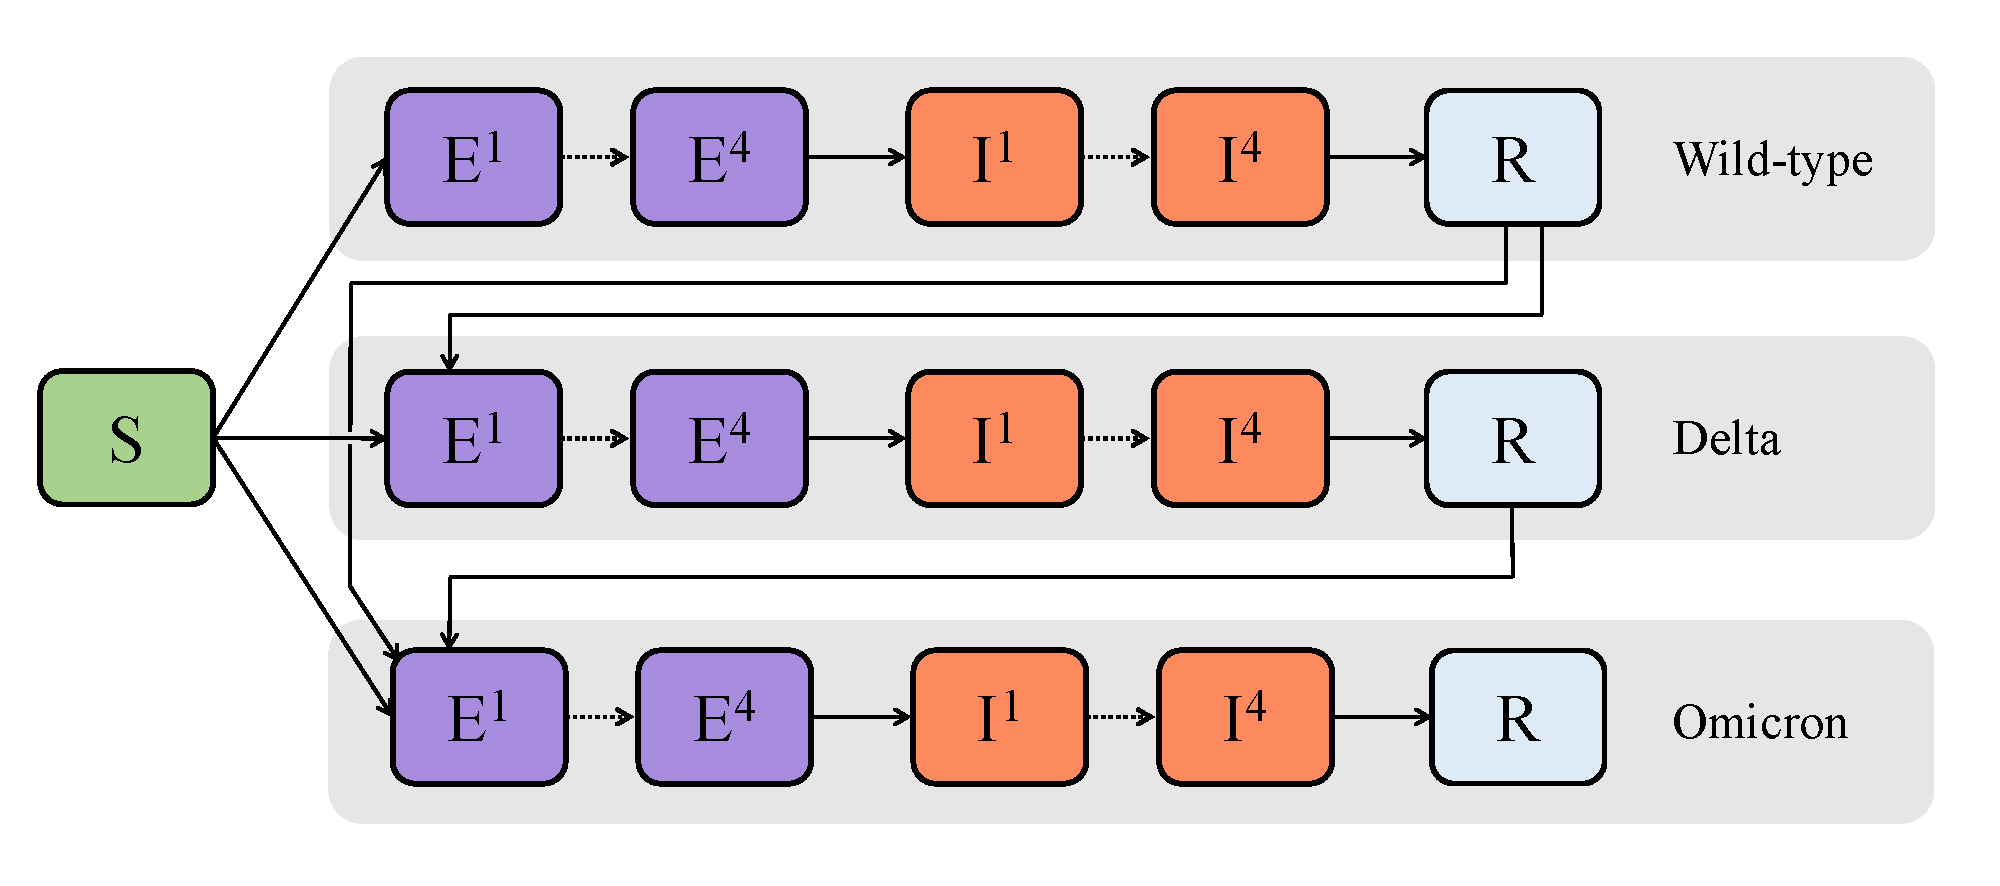
\includegraphics[width=0.75\textwidth]{../../tex_descriptions/models/sm_covid/sm_covid_se4i4r.pdf}
    \end{center}
    \caption{Compartmental model structure. 
    S = Susceptible, E = Exposed / Latent, I = Active disease, R = Recovered.
    Stratification by age and vaccination status are not shown here.
    } 
    \label{fig:se4i4r}
\end{figure}

The main rationale for using four serial compartments for both the latent and active states is to achieve an Erlang distribution for the time spent in each of these states. This distribution is more realistic than
the exponential distribution that would have been associated with a single compartment, because the Erlang distribution does not have a large density mass around 0 and is not heavy-tailed. 
The four active disease compartments have all exactly the same characteristics. However, the last two latent compartments are infectious whereas the first two are not. We further assume that 
the infectious latent compartments are half as infectious as the active disease compartments.

\subsubsection{Stratification by age}
\subsection{Model stratification}
% Note that this will vary for every application, so will need to be edited - not sure of how best to manage this:
All compartments of the base compartmental structure were stratified by age, location and organ status:\linebreak
Age
\begin{itemize}
    \item Zero to 14 years
    \item 15 to 24 years
    \item 25 to 49 years
    \item 50 to 69 years
    \item 70 years and above
\end{itemize}
Location
\begin{itemize}
    \item South Tarawa
    \item Other location
\end{itemize}
Organ status
\begin{itemize}
    \item Pulmonary smear-posivtive
    \item Pulmonary smear-negative
    \item Extrapulmonary
\end{itemize}


\subsubsection{Stratification by vaccination status}


\subsubsection{Stratification by strain}